\documentclass{article}
\usepackage{neurips_2026}
\usepackage[utf8]{inputenc}
\usepackage[T1]{fontenc}
\usepackage{hyperref}
\usepackage{url}
\usepackage{booktabs}
\usepackage{amsfonts,amsmath,amssymb,amsthm}
\usepackage{nicefrac}
\usepackage{microtype}
\usepackage{xcolor}
\usepackage{graphicx}
\usepackage{multirow}
\usepackage{enumitem}
\setlist{nosep,leftmargin=*}

\newtheorem{proposition}{Proposition}
\newtheorem{definition}{Definition}
\theoremstyle{remark}
\newtheorem{remark}{Remark}
\newcommand{\K}{K^\ast}
\newcommand{\Lm}{L^\ast}
\newcommand{\gs}{g^\ast}
\newcommand{\R}{\mathbb{R}}

\title{How Much Targeted Training Does It Take to Top a Multi-Task Leaderboard? Minimum-Investment Analysis Across Aggregation Rules}
\author{Anonymous Authors}

\begin{document}
\maketitle

\begin{abstract}
A multi-task leaderboard turns per-task scores into one ranking through an aggregation rule, and a developer can try to lift a chosen model to first place by training on data related to some of the sub-tasks. We ask what investment this takes and how it depends on the rule. We measure investment by three quantities: \emph{breadth} (number of sub-tasks improved), \emph{magnitude} (total score points gained) and \emph{depth} (largest single-task gain). We assume that rivals stay fixed and that an investment changes only the targeted sub-task's score. Under these assumptions we compute the exact minimum of each quantity for eight rules: arithmetic, geometric and harmonic mean, minimum, median, Borda, Copeland and plurality. We use closed forms for the cardinal rules and exact mixed-integer programs for the ordinal ones, and check both against brute force. We apply them to HELM-MMLU (79 models, 57 subjects) and to two views of the Open LLM Leaderboard (6 tasks; 24 BBH sub-tasks; more than 4,000 models each). We find the following. (i) The arithmetic mean is the most expensive rule in total points ($L^\ast=n\Delta$). The other seven rules need 6--94\% of that for the same targets, and the difference is significant in all 21 benchmark-by-rule comparisons (Holm-corrected $p<0.001$). (ii) The ordering by \emph{breadth} and by \emph{depth} is not stable. On the 57-task board Borda and Copeland need $2.8$--$3.8\times$ the mean's breadth, whereas on the 6-task board the rules differ by at most one task. Plurality needs $0.46\times$ the mean's depth on HELM but $1.6\times$ on the 6-task board. (iii) The requirement scales linearly with the number of tasks for the mean, but is flat for median, minimum and plurality. (iv) Whether a rule is easy to push depends on the achievable per-task gain. With gain caps taken from observed fine-tuning gains, only 15\% of contenders can reach first place under the mean, against 95--100\% under median and minimum. Requirements of the mean-type rules are stable under score noise, but the identity of the incumbent is not. Hence no aggregation rule is uniformly hardest to manipulate; the answer depends on how investment is measured. The conclusions hold under strong assumptions (static rivals, no spillover, noise-free scores), which we state and probe. Code and data checksums are provided.
\end{abstract}

\section{Introduction}
Rankings from multi-task benchmarks such as MMLU, BIG-Bench Hard, HELM and the Open LLM Leaderboard shape which models are adopted, published and funded~\citep{hendrycks2021mmlu,suzgun2023bbh,liang2022helm}. A leaderboard row is an aggregate: each model has a score on every sub-task, and an aggregation rule maps the score vector to a rank. Developers therefore have an incentive to act on the inputs of the aggregation. A direct way is to fold data related to selected sub-tasks into a model's training, which raises the model's score on those sub-tasks. Contamination of test data~\citep{zhou2023cheater,yang2023rephrased} and selective private testing~\citep{singh2025illusion} are known cases. How easily such targeted investment changes the top of a board, and whether the answer depends on the aggregation rule, has received little systematic quantitative study. Prior work compares rules by their rankings~\citep{dehghani2021lottery,lanctot2023social}, or models strategic post-training as a game~\citep{chen2026incentives}.

We take a complementary, non-game-theoretic view: \emph{measure the cheapest investment that makes a given model strictly first}, for several rules, on public boards. Our contributions are:
\begin{enumerate}
\item A \textbf{formalisation} of targeted investment with three nested cost measures: breadth $K$, magnitude $L$ and depth $g$. It includes explicit modelling assumptions and a per-task gain cap (\S\ref{sec:framework}).
\item \textbf{Exact solvers} for eight rules: closed forms or water-filling for cardinal rules, exact MILPs for Borda, Copeland and plurality. Propositions 1--4 give monotonicity, closed forms and a breadth bound. The solvers are verified against brute force on 800 random instances (\S\ref{sec:framework}, App.~\ref{app:proofs}).
\item An \textbf{empirical study} on three public boards with paired comparisons across rules, a score-noise bootstrap, a task-count scaling experiment, a synthetic latent-factor experiment that locates where conclusions flip, and a calibration of gain caps from observed fine-tuning pairs (\S\ref{sec:results}).
\item A \textbf{qualified answer}: ``it depends'', with explicit conditions. The ordering of rules changes with the cost measure, the number of tasks and the incumbent, so claims that a rule is ``robust to leaderboard gaming'' need to name the cost measure and the assumed gain ceiling.
\end{enumerate}

\section{Related work}
\textbf{Benchmark validity and leaderboard gaming.} The Benchmark Lottery shows that task selection and aggregation can reorder methods~\citep{dehghani2021lottery}. Leaderboard Illusion documents selective submission and uneven data access on Chatbot Arena~\citep{singh2025illusion}. Benchmark leakage and rephrased-sample contamination inflate scores~\citep{zhou2023cheater,yang2023rephrased}. These works establish that gaming occurs. We quantify \emph{how much of it is needed to change first place} under different rules. \citet{chen2026incentives} study equilibria of strategic post-training in a game between benchmark designers and developers; we do not model equilibrium, only the single-developer, static-rival cost. We know that work only through its title and the one-line description in the task's starter list and have not examined its results.

\textbf{Social choice and evaluation.} \citet{lanctot2023social} apply voting theory to multi-task agent evaluation, and \citet{brandt2016handbook} survey computational social choice. By Gibbard--Satterthwaite~\citep{gibbard1973manipulation,satterthwaite1975strategy}, every deterministic, onto, non-dictatorial voting rule with at least three alternatives is manipulable by voters. Our manipulation is different: the developer changes the \emph{candidate's own scores} (the ``ballots'' are task-wise rankings that move when the candidate improves). This is closest to \emph{shift/swap bribery} with costs~\citep{faliszewski2009bribery,elkind2009swap} and to manipulation complexity~\citep{bartholdi1989computational}, where cost is the number of changed votes. We differ in using real-valued scores, ties, caps and three cost measures, and in reporting empirical rather than worst-case costs. We do not claim hardness results.

\section{Framework}\label{sec:framework}
\textbf{Board and rules.} A board has $M$ models and $n$ tasks with scores $s_{mj}\in[0,U]$ ($U=100$, higher is better). Target model $t$ has score vector $a=s_{t\cdot}$; rivals $S_{-t}$ are the other $M-1$ rows. A rule $\mathcal A$ maps each row to a score or a rank. We study:
\emph{cardinal} rules (score depends only on the model's own row): arithmetic mean, geometric mean and harmonic mean (power means $p=1,0,-1$ on $s+1$, minus 1, so that zero scores are allowed), minimum, and median;
\emph{ordinal} rules (depend on cross-model comparisons per task): Borda (mean win rate, i.e.\ total number of models beaten summed over tasks), Copeland (number of rivals beaten in pairwise task-majority), and plurality (number of tasks on which a model is best, ties split). Ties are counted as one half.

\textbf{Investment.} An investment is a vector $\delta\in\R^n_{\ge0}$ with $a_j+\delta_j\le U$ and $\delta_j\le g$, where $g$ is the \emph{per-task gain cap}. It is interpreted as the score gain on task $j$ from training on data related to $j$. We use three costs:
\[
\text{breadth } K(\delta)=|\{j:\delta_j>0\}|,\qquad \text{magnitude } L(\delta)=\textstyle\sum_j\delta_j,\qquad \text{depth } \|\delta\|_\infty .
\]
$K^\ast(g)$ and $L^\ast(g)$ are the minima over investments that make $t$ \emph{strictly first} under $\mathcal A$ with rivals fixed; $g^\ast$ is the smallest cap for which any investment succeeds (the minimum depth). They are different objectives: $K^\ast$ proxies data-curation breadth, $L^\ast$ proxies total improvement effort, and $g^\ast$ the hardest single-task improvement. We report all three and never merge them into one cost.

\textbf{Assumptions.}
\textbf{(A1) Task-local effect:} an investment on task $j$ changes only $s_{tj}$ (no spillover). This favours neither low nor high costs: positive transfer would reduce $K^\ast$, negative transfer would raise it. \textbf{(A2) Static rivals:} other rows do not change, so the results are a one-shot, best-response-free cost. \textbf{(A3) Gain cap:} $g$ bounds per-task improvement; we sweep $g$ and calibrate it from observed fine-tuning pairs (\S\ref{sec:calib}). \textbf{(A4) Noise-free scores:} the published numbers are taken as the truth; relaxed by a bootstrap (\S\ref{sec:noise}). \textbf{(A5) Strictness:} the target must exceed every rival by a margin $\epsilon=10^{-6}$ points on the aggregate (cardinal) or $10^{-3}$ points on a task (ordinal), so ties never count as wins.

\begin{proposition}[Monotonicity]\label{prop:mono}
For all eight rules, if $\delta$ makes $t$ strictly first then so does any $\delta'\ge\delta$ within the caps. Hence (i) a cap $g$ is feasible iff the all-in investment $\delta_j=\min(g,U-a_j)$ succeeds; (ii) feasible caps form an up-set $[g^\ast,\infty)$, so $g^\ast$ is found by bisection; (iii) $K^\ast(g)$ and $L^\ast(g)$ are non-increasing in $g$.
\end{proposition}
\begin{proposition}[Mean]\label{prop:mean}
Let $\Delta=T+\epsilon-\bar a$, where $T$ is the best rival mean, and $c_j=\min(g,U-a_j)$. If $\sum_jc_j\ge n\Delta$ then $L^\ast=n\Delta$ (independent of $g$), $K^\ast=\min\{k:\text{sum of the }k\text{ largest }c_j\ge n\Delta\}\ge\lceil n\Delta/g\rceil$, and $g^\ast\ge\Delta$ with equality if no ceiling binds. Otherwise the target cannot win.
\end{proposition}
\begin{proposition}[Minimum]\label{prop:min}
With $T$ the best rival minimum, $K^\ast=|\{j:a_j<T+\epsilon\}|$, $L^\ast=\sum_j(T+\epsilon-a_j)_+$ and $g^\ast=\max_j(T+\epsilon-a_j)_+$. $K^\ast$ does not depend on $g$: breadth cannot be traded for depth under this rule.
\end{proposition}
\begin{proposition}[Order statistics]\label{prop:order}
Let the rule be the $r$-th largest task score, $r=\lceil (n+1)/2\rceil$ for the median with odd $n$, and let $m=|\{j:a_j\ge T+\epsilon\}|$. Then $K^\ast=\max(0,r-m)\le r$, and $L^\ast$ is the sum of the $r-m$ smallest reachable deficits. For even $n$ the median averages ranks $n/2$ and $n/2+1$ and $K^\ast\le n/2+1$. Breadth is thus bounded by about half the tasks, whatever the gap.
\end{proposition}
Proofs are in App.~\ref{app:proofs}. Proposition~\ref{prop:mean} gives the main scaling prediction: at a fixed aggregate gap, the mean's total points grow linearly with $n$, whereas Proposition~\ref{prop:order} gives a bound that does not grow with the gap.

\textbf{Algorithms.} Cardinal rules use the closed forms above (geometric and harmonic means by greedy selection of the largest gains for $K^\ast$, and water-filling for $L^\ast$; the median uses an exact breakpoint search). Ordinal rules are solved as exact MILPs (HiGHS via SciPy) over discrete ``level'' choices: for each task the target either keeps its score or rises to just above one rival's score (the only useful levels). We minimise $K$ or $L$ subject to strict first place, with a 60\,s limit (optimality flags were recorded in the main sweep, where no instance hit the limit). The correctness check in \texttt{code/test\_lib.py} compares every solver with brute-force enumeration (integer boards, 120 cardinal trials $\times$ 3 rules; 60 ordinal boards $\times$ 3 rules $\times$ 2 objectives) and SLSQP with subset enumeration for geometric/harmonic means (40 boards): 0 mismatches.

\section{Experimental setup}\label{sec:setup}
\textbf{Boards.} (1) \textbf{HELM-MMLU}: HELM release v1.13.0 (2025-01-10), exact-match accuracy on 57 MMLU subjects, 79 models with complete data~\citep{helm_release}. (2) \textbf{OLLB-6}: the Open LLM Leaderboard \texttt{contents} snapshot (commit 9c09a7c, 2025-03-20), six normalised task scores (IFEval, BBH, MATH Lvl 5, GPQA, MUSR, MMLU-PRO), 4,442 models after removing the one flagged model and models with an identical score vector~\citep{ollb_contents}. (3) \textbf{OLLB-BBH24}: the 24 BBH sub-task accuracies from the \texttt{results} snapshot (commit aa81ecc), latest file per model, 4,403 models after de-duplication~\citep{ollb_results}; their mean agrees with the \texttt{BBH Raw} column of the other snapshot (correlation $0.9996$). Licences are not declared for the score data; we use only aggregate scores (App.~\ref{app:repro}). Cardinal rules use the full board. Ordinal MILPs use the top-100 models by arithmetic mean for the two OLLB boards, to bound solver size; this changes the rival set for those rules (limitation).

\textbf{Targets.} We take the model ranked $r$ under the rule in question. We use ranks $r=2$--$11$ (``contenders'') for the cap sweeps and the noise and scaling studies, ranks $2$--$21$ for ordinal rules (solver cost) in the rank sweep, and, for \emph{paired} comparisons across rules, a common target set: ranks $2$--$31$ by arithmetic mean (30 models), so every rule is evaluated on the same models. A target that is already first under the rule or under the mean is dropped from that pair.

\textbf{Statistics.} Summaries are medians with inter-quartile ranges over targets; targets are not independent random draws, so intervals describe heterogeneity across contenders and not sampling error of the board. Paired comparisons use Wilcoxon signed-rank tests of (rule $-$ mean) over common targets, Holm-corrected over the 7 non-reference rules within each benchmark and metric, and a 10,000-sample bootstrap over targets for the median paired ratio. There are three boards, so we make no claim about generalisation across boards beyond what the three show. The study was developed with early exploratory runs on HELM-MMLU, so all analyses should be read as exploratory; we did not hold out a confirmatory board. Seeds, commands and timings are in App.~\ref{app:repro}.

\section{Results}\label{sec:results}
Descriptives of the boards are in Table~\ref{tab:desc}. The winner differs across rules on every board (App.~\ref{app:more}): on HELM, Claude 3.5 Sonnet (2024-10-22) wins under mean, Borda and Copeland, DeepSeek v3 under geometric/harmonic mean, minimum and median, and Claude 3.5 Sonnet (2024-06-20) under plurality. On OLLB-6 the winners also differ. Kendall's $\tau$ between mean and plurality scores (over the ordinal pool) is $0.51$ (HELM) and $0.17$ (OLLB-6). Therefore the choice of rule matters for who is the \emph{incumbent} a contender has to beat, which we return to below.

\begin{table}[t]
\centering\small
\caption{Boards. ``Ordinal pool'' is the number of models used for ordinal rules; ``Add.\ resid.\ SD'' is the residual SD (points) of a two-way additive fit (model + task), i.e.\ the task-specific variation that is not a model-wide skill effect.}\label{tab:desc}
\begin{tabular}{lrrrrr}\toprule
Board & Models & Tasks & Ordinal pool & SD of model means & Add. resid. SD\\\midrule
HELM-MMLU & 79 & 57 & 79 & 9.9 & 5.8\\
OLLB-6 & 4442 & 6 & 100 & 10.8 & 9.2\\
OLLB-BBH24 & 4403 & 24 & 100 & 11.4 & 9.5\\
\bottomrule\end{tabular}

\end{table}

\subsection{Comparing rules on the same targets}
Table~\ref{tab:paired} gives the median over the 30 common targets of the ratio (requirement under the rule)/(requirement under the mean), with the mean's absolute value for reference; Table~\ref{tab:summary} (App.) lists medians and IQRs per rule for rank 2--11 contenders, and Fig.~\ref{fig:rank} shows the requirement as a function of rank.

\begin{table}[t]
\centering\small
\caption{Paired comparison on 30 common targets (ranks 2--31 by mean). Entries: median ratio of the requirement under the rule to that under the arithmetic mean ($<1$: easier than the mean). Cap $g{=}100$ for $L^\ast,K^\ast$. $^\dagger$: not significant after Holm correction (Wilcoxon, $\alpha=0.05$); all other entries have $p_{\rm Holm}<0.05$. CIs, shares and $p$-values in App.~\ref{app:more}, Table~\ref{tab:pairedfull}.}\label{tab:paired}
\resizebox{\textwidth}{!}{\begin{tabular}{lccccccccc}\toprule
 & \multicolumn{3}{c}{Magnitude $L^*$ ($g{=}100$)} & \multicolumn{3}{c}{Breadth $K^*$ ($g{=}100$)} & \multicolumn{3}{c}{Depth $g^*$}\\
\cmidrule(lr){2-4}\cmidrule(lr){5-7}\cmidrule(lr){8-10}
Rule & HELM & OLLB-6 & BBH24 & HELM & OLLB-6 & BBH24 & HELM & OLLB-6 & BBH24\\\midrule
Geometric & 0.94 & 0.73 & 0.90 & 1.00$^{\dagger}$ & 1.00$^{\dagger}$ & 1.00$^{\dagger}$ & 1.08 & 1.19 & 1.11\\
Harmonic & 0.89 & 0.57 & 0.80 & 1.00$^{\dagger}$ & 1.00$^{\dagger}$ & 1.00$^{\dagger}$ & 1.18 & 1.29 & 1.23\\
Minimum & 0.09 & 0.40 & 0.27 & 0.64 & 2.00 & 1.00$^{\dagger}$ & 1.81 & 1.59 & 2.11\\
Median & 0.09 & 0.13 & 0.13 & 1.31 & 1.00$^{\dagger}$ & 1.00$^{\dagger}$ & 0.75 & 0.39 & 0.82\\
Borda & 0.63 & 0.24 & 0.08 & 3.80 & 1.00 & 1.20 & 0.98$^{\dagger}$ & 0.42 & 0.16\\
Copeland & 0.25 & 0.27 & 0.24 & 2.84 & 2.00 & 1.50 & 0.72 & 0.76 & 1.31\\
Plurality & 0.06 & 0.37 & 0.30 & 1.00$^{\dagger}$ & 2.00 & 1.75 & 0.46 & 1.57 & 1.13\\
\midrule
Mean (abs., ref.) & 379.9 & 31.9 & 242.4 & 9.0 & 1.0 & 4.0 & 7.3 & 5.3 & 11.0\\
\bottomrule\end{tabular}
}
\end{table}

\textbf{Magnitude.} All 21 ratios are below 1 and highly significant: the mean is the most expensive rule in total points on every board, as predicted by $L^\ast=n\Delta$. Geometric and harmonic means save only 6--43\%. The median, minimum, Copeland and plurality need 6--40\%, and Borda 8--63\%. A plausible reason, which our experiments do not isolate, is that mean-type rules require the target's \emph{whole-board} aggregate to move, whereas rank-based rules only need changes at the few tasks where the target loses to its rival.

\textbf{Breadth.} The picture reverses. On HELM, Borda needs $3.8\times$ and Copeland $2.8\times$ the mean's breadth (medians $34.5$ and $27$ tasks against $9$ for the mean, out of 57), while the minimum needs $0.64\times$ and the median $1.3\times$; geometric, harmonic and plurality are indistinguishable from the mean. On OLLB-6 every rule needs one or two tasks, so the ratios are $1$--$2$ and represent a difference of a single task. On BBH24, Copeland and plurality need $1.5$--$1.75\times$. A plausible reason, again not isolated, is that a pairwise-majority or win-count rule asks the target to beat \emph{many} rivals, each on a majority of tasks, whereas a mean only asks it to cover a sum.

\textbf{Depth.} The ordering by minimum depth $\gs$ is unstable across boards. Plurality needs $0.46\times$ the mean's depth on HELM, but $1.57\times$ on OLLB-6 and $1.13\times$ on BBH24. Copeland needs $0.72\times$, $0.76\times$ and $1.31\times$. Geometric and harmonic means need slightly \emph{more} depth than the mean everywhere ($1.08$--$1.29\times$), since low scores are weighted more and gains on already-high tasks count less. The minimum needs $1.6$--$2.1\times$ the mean's depth. The Borda ratio on BBH24 ($0.16\times$) reflects that Borda's incumbent there is a different, weaker model than under the other rules (Table~\ref{tab:winners}): paired comparisons fix the target but not the incumbent.

\begin{figure}[t]
\centering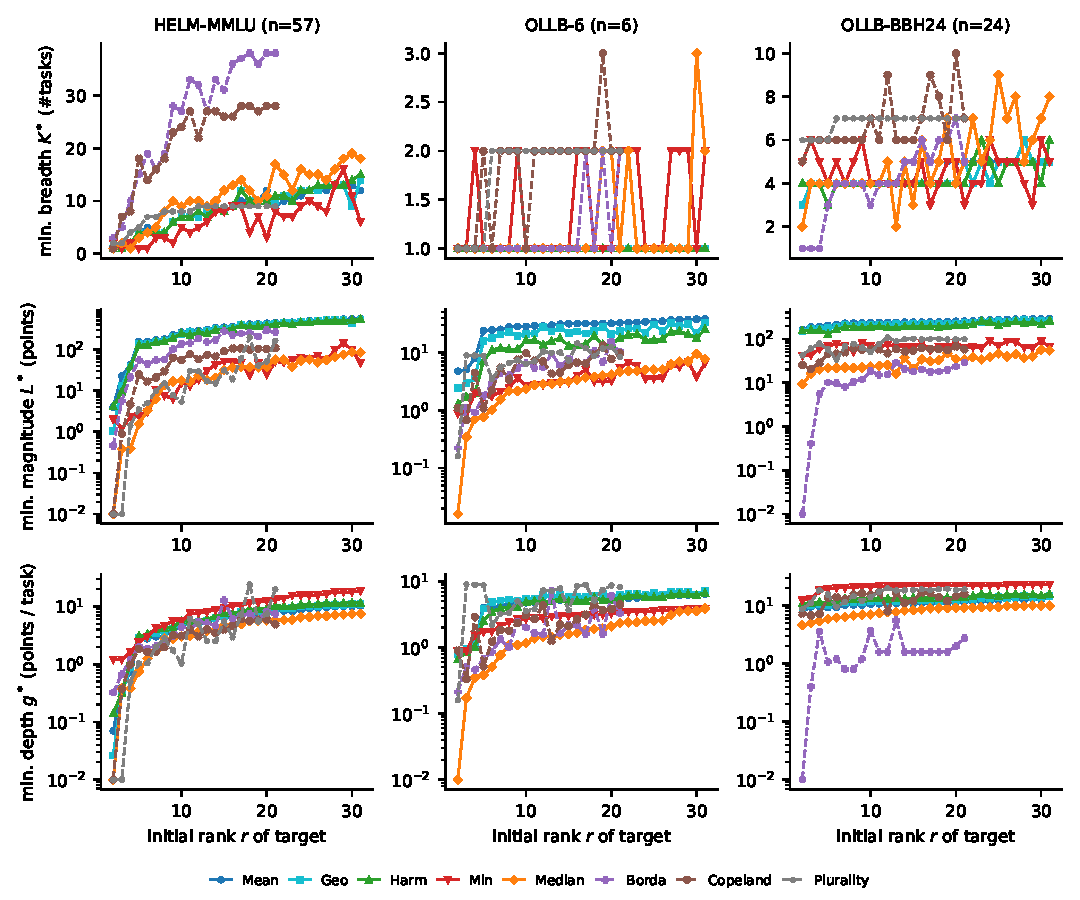
\includegraphics[width=\textwidth]{figs/fig_rank_sweep.pdf}
\caption{Minimum investment to become first versus the target's initial rank under each rule (uncapped gains, $g=100$). Rows: breadth $\K$, magnitude $\Lm$ (log), depth $\gs$ (log). Solid: cardinal; dashed: ordinal rules (ranks up to 21). The requirement of the mean rises steeply in magnitude, while for the minimum, median and plurality it stays small.}\label{fig:rank}
\end{figure}

\subsection{Scaling with the number of tasks}\label{sec:scaling}
On HELM we repeatedly draw $m\in\{6,12,24,40\}$ of the 57 subjects (60 draws each) and recompute everything, including who the contenders are (Fig.~\ref{fig:subsample}). The mean's magnitude per task is flat at about $3$ points ($=\Delta$), i.e.\ $\Lm$ grows linearly with $m$ as in Proposition~\ref{prop:mean}; the median's and minimum's $\Lm$ are flat or decreasing in absolute terms (median $\approx5$ points at every $m$). Borda and Copeland breadth grow roughly linearly with $m$ ($3\to12$ tasks from $m=6$ to $40$, and $17$ at $m=57$), whereas mean breadth grows slowly ($1\to3$). So the \emph{relative cost of rules depends on board size}: Borda and Copeland need about 3 tasks against the mean's 1 at $m=6$, but 12 against 3 at $m=40$, so the absolute gap widens from 2 to 9 tasks.

\begin{figure}[t]
\centering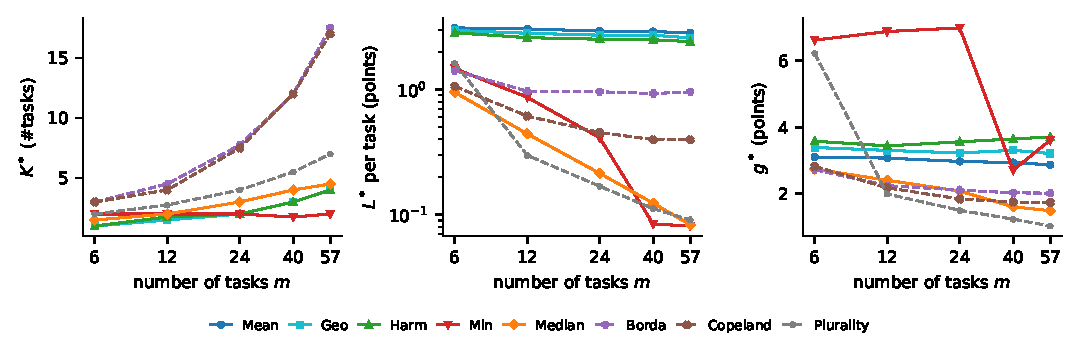
\includegraphics[width=\textwidth]{figs/fig_subsample.pdf}
\caption{Task-subsampling on HELM-MMLU (median over 60 random subsets per $m$ and over contenders of rank 2--11; the point at $m=57$ is the full board). Left: breadth. Middle: magnitude per task. Right: depth.}\label{fig:subsample}
\end{figure}

\subsection{When do conclusions flip? A synthetic latent-factor study}
To locate the mechanism, we generate boards $s_{mj}=\mathrm{clip}_{[0,100]}(60+\theta_m+b_j+\sigma\varepsilon_{mj})$ with $M=80$, $\theta_m\sim N(0,10^2)$, $b_j\sim N(0,8^2)$ and task-specific noise SD $\sigma\in\{1,2,4,8,16\}$ (40 boards per cell, $n\in\{12,57\}$; Fig.~\ref{fig:synth}). The empirical boards have additive residual SD of $5.8$--$9.5$ points (Table~\ref{tab:desc}), inside this range. At $n=57$, as $\sigma$ grows from 1 to 16, Borda's relative breadth $K^\ast/n$ falls from $0.79$ to $0.17$ and plurality's from $0.46$ to $0.07$, while the mean's falls only from $0.29$ to $0.17$; at $\sigma=1$ (nearly one-dimensional board) Borda must touch most tasks, since a target behind a rival is behind on almost every task. Magnitude per task stays near $8$--$10$ points for the mean at all $\sigma$ but falls for rank-based rules. The synthetic boards are an illustration of the mechanism and not evidence about real boards.

\begin{figure}[t]
\centering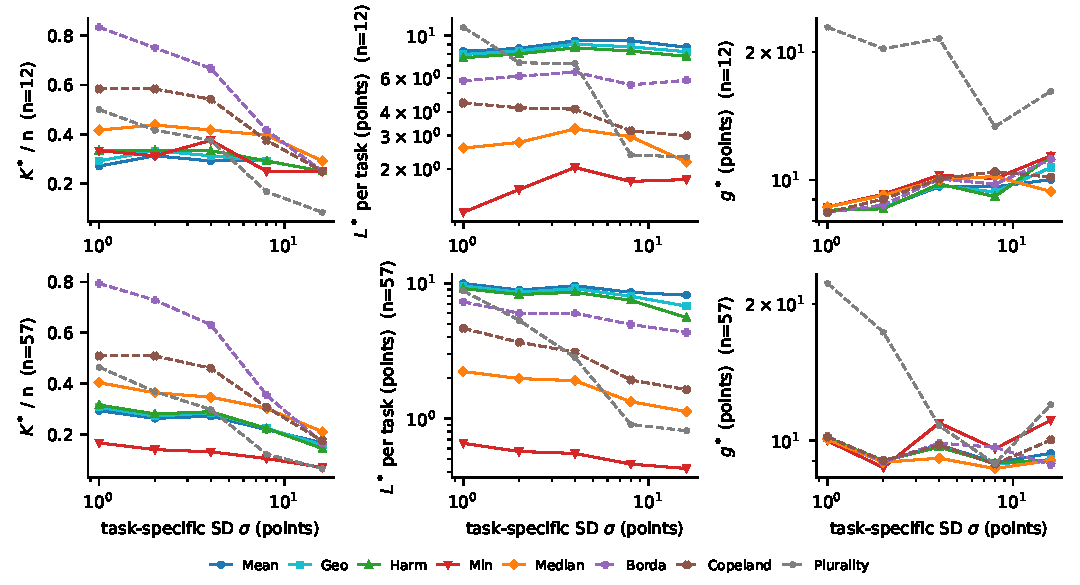
\includegraphics[width=\textwidth]{figs/fig_synthetic.pdf}
\caption{Synthetic boards (median over 40 boards and over contenders of rank 2--11). Top: $n=12$; bottom: $n=57$. Left: relative breadth $K^\ast/n$; middle: magnitude per task; right: depth $\gs$. Cap $g=100$.}\label{fig:synth}
\end{figure}

\subsection{Robustness to score noise}\label{sec:noise}
HELM reports accuracies on 100--1,534 instances per subject. We re-draw every cell as $\mathrm{Binomial}(n_{\rm eval},p)/n_{\rm eval}$ around the observed accuracy (100 draws) and recompute everything including contender identity (Table~\ref{tab:noise} in the App.). The median requirement of mean-type rules is tight ($K^\ast$ 95\% interval width 2--2.5 tasks; $\Lm$ about $\pm20\%$), whereas the minimum, median and plurality vary widely ($\Lm$ for the minimum 3.1--35.8; for the median 2.9--14.3), since they depend on a few extreme cells. The \emph{incumbent} is unstable: the observed winner stays first in only 18--71\% of draws (mean $0.51$, median $0.18$, plurality $0.18$, Borda $0.68$, Copeland $0.71$). For Borda and Copeland the observed $\K$ ($17.5$ and $17$) is above the bootstrap 95\% interval ($7$--$14.5$ and $9$--$15.5$): the observed board is more ``consistently ordered'' across tasks than a noisy replicate, so ordinal requirements are sensitive to noise. The bootstrap is centred on already-noisy observed values, so it adds noise on top of noise and is a sensitivity check, not a calibrated error bar.

\subsection{Realistic gain caps}\label{sec:calib}
Everything above that uses $g=100$ is the least restrictive case for feasibility. We calibrate caps with naturally occurring gains in the Open LLM Leaderboard: for 88 non-merged, original-weight models whose declared base model is itself a fine-tuned or chat model on the board, we compute (fine-tuned $-$ base) per task, and take the per-task 90th percentile, 99th percentile and maximum as caps (App., Table~\ref{tab:calib}). With caps from this primary pair set, on OLLB-6 only $15\%$ (mean), $25\%$ (geometric) and $10\%$ (plurality) of the contenders at ranks 2--21 can reach first place with q90 caps, against $90\%$ (harmonic), $95\%$ (median), $100\%$ (minimum), $80\%$ (Borda) and $75\%$ (Copeland); with q99 caps all contenders succeed under every rule (Table~\ref{tab:calibfeas}). When the 480 pairs that include base$\to$instruct jumps are used, q90 caps (which reach 41 points on IFEval) already suffice for nearly everyone ($55$\% for plurality, $90$\% for Copeland, $100$\% otherwise). \emph{The apparent robustness of a rule thus depends on the assumed gain ceiling more than on the rule}. Gains are not automatic: in the primary pair set the median gain is at most $1.6$ points (negative on five of six tasks) and only 19--74\% of pairs gain on a given task.

\begin{table}[t]
\centering\small
\caption{Fraction of ranks 2--21 on OLLB-6 that can reach first place when each task's gain is capped at the q90/q99/maximum of observed fine-tuning gains.}\label{tab:calibfeas}
\begin{tabular}{lcccccc}\toprule
 & \multicolumn{3}{c}{tuned$\to$tuned pairs (88)} & \multicolumn{3}{c}{all pairs (480)}\\\cmidrule(lr){2-4}\cmidrule(lr){5-7}
Rule & q90 & q99 & max & q90 & q99 & max\\\midrule
Mean & 0.15 & 1.00 & 1.00 & 1.00 & 1.00 & 1.00\\
Geometric & 0.25 & 1.00 & 1.00 & 1.00 & 1.00 & 1.00\\
Harmonic & 0.90 & 1.00 & 1.00 & 1.00 & 1.00 & 1.00\\
Minimum & 1.00 & 1.00 & 1.00 & 1.00 & 1.00 & 1.00\\
Median & 0.95 & 1.00 & 1.00 & 1.00 & 1.00 & 1.00\\
Borda & 0.80 & 1.00 & 1.00 & 1.00 & 1.00 & 1.00\\
Copeland & 0.75 & 1.00 & 1.00 & 0.90 & 1.00 & 1.00\\
Plurality & 0.10 & 1.00 & 1.00 & 0.55 & 1.00 & 1.00\\
\bottomrule\end{tabular}

\end{table}

\subsection{An observed case}
On OLLB-BBH24 the incumbent under seven of eight rules is \texttt{qingy2024/Benchmaxx-Llama-3.2-1B-Instruct} (mean $82.7$), whose declared parent \texttt{meta-llama/Llama-3.2-1B-Instruct} is also on the board (mean $35.0$). The child improves on the parent on \emph{all} 24 sub-tasks, by $16.4$--$68.4$ points, a total of $1145$ points. The same child has IFEval $20.1$ and MMLU-PRO $1.3$ (OLLB-6 columns), so its gain is concentrated on BBH. Table~\ref{tab:case} compares this observed gain with the minimum our solvers need for the parent to be strictly first against the field without the child: $13$ tasks and $981$ points under the mean (the observed gain is about $17\%$ above the minimum in magnitude and touches nearly twice as many tasks), and fewer than half the points under the median, minimum, Copeland and plurality rules. This is descriptive: we have no information about how the child was trained, the model name is suggestive only, and a single case shows that our requirements are the right order of magnitude and not that they were what the developer targeted.

\begin{table}[t]
\centering\small
\caption{Case study on OLLB-BBH24: observed gain of the incumbent over its parent vs.\ the minimum investment the parent needs for strict first place (cap $g=100$).}\label{tab:case}
\begin{tabular}{lrr}\toprule
 & Breadth $K$ & Magnitude $L$ (points)\\\midrule
Observed parent$\to$child gain & 24 & 1145\\\midrule
Minimum needed, Mean & 13 & 981\\
Minimum needed, Geometric & 14 & 898\\
Minimum needed, Harmonic & 14 & 823\\
Minimum needed, Minimum & 17 & 250\\
Minimum needed, Median & 12 & 441\\
Minimum needed, Borda & 18 & 662\\
Minimum needed, Copeland & 13 & 431\\
Minimum needed, Plurality & 4 & 88\\
\bottomrule\end{tabular}

\end{table}

\section{Discussion and limitations}
\textbf{Answer to the research question.} Under static rivals and task-local effects, topping these boards from rank 2--11 needs only a few tasks (median $K^\ast$ 1--4 for the mean-type rules, up to 17 for Borda/Copeland on HELM) when per-task gains are unlimited, but the \emph{total} improvement is large for the mean (about 160 points on HELM, i.e.\ roughly $3$ points on every task, or $\ge 16$ tasks at a cap of $10$). The dependence on the rule is real but not a ranking: the mean is the costliest in magnitude; rank-based rules are cheaper in magnitude but can be costlier in breadth; depth flips with the board. Conclusions about ``which rule resists gaming'' are therefore conditional on (i) the cost measure, (ii) the number of tasks and the amount of task-specific variation, (iii) the incumbent and (iv) the assumed ceiling on per-task gains.

\textbf{Limitations.} (1) \emph{Static rivals and one developer:} real boards are repeated games and rivals respond; our numbers are a one-shot cost, not an equilibrium. (2) \emph{No spillover (A1):} training on one subject can lift related subjects (HELM-MMLU subjects are strongly correlated), which would lower $K^\ast$ under the real process; the minimal $K^\ast$ is a lower bound only under A1. (3) \emph{Scores as cost proxy:} we have no model of how many training examples a point of gain costs, so magnitude is only a proxy and we do not say which cost measure is the ``right'' one. (4) \emph{Noise-free scores} (partly addressed in \S\ref{sec:noise}); HELM subjects have as few as 100 items. (5) \emph{Three boards}, all language-model benchmarks; the OLLB boards contain many near-duplicate fine-tunes and merges, and we use the top-100 pool for ordinal rules there, which changes the rival set. OLLB-6 scores are normalised so that random-guess accuracy maps to 0, which affects geometric and harmonic means (we add 1 to scores before taking them). (6) \emph{Calibration:} caps are derived from 88 pairs (480 in a sensitivity run), are the same for every target and ignore that gains saturate near the ceiling. (7) \emph{Exploratory design:} early pilots on HELM informed the study; there is no preregistered confirmatory board, and 3 boards $\times$ 8 rules do not support a statement about all boards. (8) Intervals over contenders describe heterogeneity, not sampling error. (9) The exact MILPs are not claimed to scale beyond the board sizes used. Solver optimality flags were checked only in the main sweep (no time-limit hits there); the Monte-Carlo studies use 20--30\,s limits and did not record them.

\textbf{Broader impact.} The analysis could inform benchmark designers who choose aggregation rules and could in principle guide a developer wishing to game a board. We believe the former use dominates: the study is based on public scores and makes no claim about specific developers (the case study is descriptive and stated as such). We discuss no data or models with misuse risk. We recommend reporting results under several rules and reporting breadth, magnitude and depth together.

\bibliographystyle{plainnat}
\bibliography{refs}

\appendix
\section{Proofs}\label{app:proofs}
\textbf{Proposition~\ref{prop:mono}.} Raising $a_j$ weakly raises the target's aggregate under the mean, power means, minimum and median, and does not change any rival's cardinal score. For ordinal rules, let $\delta'\ge\delta$. On each task, the target beats a (weakly) larger set of rivals, so its Borda score $\sum_j\#\{\text{beaten}\}$ and each pairwise win count weakly increase, and each rival's win count against the target weakly decreases while its comparisons against other rivals are unchanged. Copeland scores follow: the target's pairwise wins against each rival can only change from loss to tie to win, and every rival's Copeland score only loses points against the target. Plurality credit of the target on task $j$ is $1/\#\text{ties}$ if it is tied-best and 1 if strictly best, which is weakly increasing in $a_j$, while every rival's credit on $j$ is weakly decreasing. Hence strict first place is preserved. (i) follows because the all-in vector is the largest feasible $\delta$; (ii) because a larger cap enlarges the feasible box; (iii) because the feasible set of a larger cap contains that of a smaller cap. \hfill$\square$

\textbf{Proposition~\ref{prop:mean}.} Winning is equivalent to $\sum_j\delta_j\ge n\Delta$ with $0\le\delta_j\le c_j$. The minimum $\ell_1$ norm of a feasible $\delta$ is $n\Delta$, attained whenever $\sum_jc_j\ge n\Delta$. The support is minimal when the coordinates with the largest caps are used; the size $k$ is the smallest with $\sum_{i\le k}c_{(i)}\ge n\Delta$. Since each $c_j\le g$, $k\ge n\Delta/g$. For $g^\ast$: $\sum_j\min(g,U-a_j)\ge n\Delta$ requires $g\ge\Delta$ since $\sum_j\min(g,\cdot)\le ng$, with equality when no ceiling binds. \hfill$\square$

\textbf{Proposition~\ref{prop:min}.} The minimum is $\ge T+\epsilon$ iff every coordinate is, so each coordinate with $a_j<T+\epsilon$ must be raised by at least $T+\epsilon-a_j$ and the others need nothing. Feasibility at cap $g$ iff $\max_j(T+\epsilon-a_j)_+\le g$ (and $T+\epsilon\le U$). \hfill$\square$

\textbf{Proposition~\ref{prop:order}.} The $r$-th largest value is $\ge T+\epsilon$ iff at least $r$ coordinates are. Of these, $m$ already are, so $r-m$ coordinates must be raised, the cheapest being the $r-m$ smallest deficits among reachable coordinates. The bound $K^\ast\le r$ is immediate. For the even-$n$ median (the mean of ranks $n/2$ and $n/2+1$): given any winning $\delta$, let $I$ be the $n/2+1$ coordinates with the largest final scores and set $\delta_j=0$ for $j\notin I$. The values in $I$ are unchanged, and the others fall but stay below the $(n/2+1)$-th largest value, so both order statistics are unchanged and the new $\delta$ still wins; hence $K^\ast\le n/2+1$. The same argument gives $K^\ast\le r$ for a general rank $r$. \hfill$\square$

\textbf{Exactness of the ordinal MILPs.} For each task only levels equal to a rival's score plus $10^{-3}$ can change an outcome; every other level costs more without changing a comparison. The binary choice of one level per task, together with linear constraints on the target's Borda/Copeland/plurality score against each rival's updated score, encodes strict first place exactly. Copeland needs auxiliary binaries for ``beaten'' and ``tied or beaten'' per rival. The match with brute force (App.~\ref{app:repro}) validates the encoding.

\section{Additional results}\label{app:more}
\begin{table}[h]
\centering\small
\caption{Median [IQR] of the requirement over contenders ranked 2--11 under each rule, with the best-rival gap $g^\ast$ (depth), breadth $K^\ast$ and magnitude $L^\ast$ (cap 100) and breadth at cap $10$ (``feas.'': share of contenders for which first place is reachable). Source: \texttt{code/02\_main.py}.}\label{tab:summary}
\resizebox{\textwidth}{!}{\begin{tabular}{llcccc}\toprule
Benchmark & Rule & $g^*$ & $K^*$ ($g{=}100$) & $K^*$ ($g{=}10$) & $L^*$ ($g{=}100$)\\\midrule
HELM-MMLU (n=57) & Mean & 2.9 [1.2, 3.7] & 4.0 [1.8, 5.8] & 16.5 [7.8, 21.8] & 161.9 [69.8, 210.9]\\
 & Geo & 3.2 [1.4, 4.0] & 4.0 [2.5, 5.5] & 16.0 [6.8, 20.2] & 147.3 [63.4, 192.4]\\
 & Harm & 3.7 [1.6, 4.3] & 4.0 [2.5, 5.5] & 15.5 [6.5, 19.5] & 137.7 [60.0, 177.5]\\
 & Min & 3.6 [1.8, 5.4] & 2.0 [1.2, 3.0] & 2.0 [1.2, 3.0] & 4.6 [2.3, 9.7]\\
 & Median & 1.5 [0.5, 2.8] & 4.5 [2.2, 8.8] & 4.5 [2.2, 8.8] & 4.7 [0.7, 15.8]\\
 & Borda & 2.0 [1.4, 2.9] & 17.5 [11.2, 25.0] & 19.5 [12.2, 27.8] & 54.6 [26.7, 89.5]\\
 & Copeland & 1.7 [1.1, 2.8] & 17.0 [9.5, 21.8] & 17.0 [9.5, 21.8] & 22.6 [7.6, 48.9]\\
 & Plurality & 1.0 [0.6, 1.9] & 7.0 [4.2, 8.0] & 7.0 [4.2, 8.0] & 5.2 [1.9, 9.2]\\
\midrule
OLLB-6 (n=6) & Mean & 4.2 [2.0, 4.7] & 1.0 [1.0, 1.0] & 3.0 [1.5, 3.0] & 25.0 [11.9, 28.1]\\
 & Geo & 5.0 [1.8, 5.3] & 1.0 [1.0, 1.0] & 2.0 [1.2, 3.0] & 18.8 [6.8, 20.8]\\
 & Harm & 3.7 [1.4, 4.1] & 1.0 [1.0, 1.0] & 2.0 [1.0, 2.0] & 11.2 [3.3, 12.0]\\
 & Min & 1.9 [1.6, 2.6] & 1.0 [1.0, 1.0] & 1.0 [1.0, 1.0] & 2.1 [1.7, 2.6]\\
 & Median & 0.6 [0.4, 1.1] & 1.0 [1.0, 1.0] & 1.0 [1.0, 1.0] & 1.3 [0.7, 2.2]\\
 & Borda & 0.9 [0.6, 1.6] & 1.0 [1.0, 1.0] & 1.0 [1.0, 1.0] & 3.5 [1.3, 5.1]\\
 & Copeland & 1.8 [1.0, 2.6] & 1.5 [1.0, 2.0] & 2.0 [1.0, 2.0] & 3.9 [1.4, 6.9]\\
 & Plurality & 3.7 [3.3, 7.9] & 2.0 [1.0, 2.0] & 2.0 [1.0, 2.0] & 6.9 [5.7, 8.5]\\
\midrule
OLLB-BBH24 (n=24) & Mean & 9.9 [9.4, 10.3] & 4.0 [4.0, 4.0] & 21.0 [20.0, 21.0] (50\% feas.) & 219.4 [194.1, 231.1]\\
 & Geo & 11.0 [10.3, 11.6] & 4.0 [4.0, 4.0] & 20.0 [20.0, 20.0] (10\% feas.) & 195.4 [176.0, 206.5]\\
 & Harm & 12.5 [11.4, 13.1] & 4.0 [4.0, 4.0] & infeasible & 172.2 [158.4, 189.4]\\
 & Min & 20.4 [18.7, 21.1] & 5.0 [4.0, 5.0] & infeasible & 66.4 [53.1, 70.4]\\
 & Median & 6.3 [5.5, 7.0] & 4.0 [4.0, 4.0] & 4.0 [4.0, 4.0] & 21.7 [20.4, 22.4]\\
 & Borda & 1.1 [0.8, 1.5] & 3.5 [1.5, 4.0] & 4.0 [1.8, 4.0] & 9.9 [6.1, 11.5]\\
 & Copeland & 13.8 [8.7, 15.5] & 6.0 [6.0, 6.0] & 6.0 [5.5, 6.0] (30\% feas.) & 48.0 [32.8, 57.7]\\
 & Plurality & 13.0 [11.3, 15.4] & 7.0 [6.0, 7.0] & 8.0 [8.0, 8.0] (20\% feas.) & 62.1 [52.1, 74.3]\\
\bottomrule\end{tabular}
}
\end{table}

\begin{table}[h]
\centering\footnotesize
\caption{Full paired comparison vs.\ the arithmetic mean (common targets, ranks 2--31 by mean), magnitude $L^\ast$; share lower . higher: fraction of targets whose requirement under the rule is lower . higher than under the mean; $p_{\rm Holm}$: Wilcoxon signed-rank, Holm-corrected over the 7 rules within benchmark and metric.}\label{tab:pairedfull}
\begin{tabular}{llrccc}\toprule
Benchmark & Rule & pairs & median ratio [95\% CI] & share lower . higher & $p_{\rm Holm}$\\\midrule
HELM-MMLU & Geometric & 29 & 0.94 [0.93, 0.95] & 1.00 . 0.00 & <0.001\\
 & Harmonic & 29 & 0.89 [0.88, 0.90] & 1.00 . 0.00 & <0.001\\
 & Minimum & 29 & 0.09 [0.07, 0.11] & 1.00 . 0.00 & <0.001\\
 & Median & 30 & 0.09 [0.07, 0.11] & 1.00 . 0.00 & <0.001\\
 & Borda & 30 & 0.63 [0.57, 0.66] & 0.97 . 0.03 & <0.001\\
 & Copeland & 30 & 0.25 [0.22, 0.27] & 1.00 . 0.00 & <0.001\\
 & Plurality & 29 & 0.06 [0.05, 0.06] & 1.00 . 0.00 & <0.001\\
\midrule
OLLB-6 & Geometric & 30 & 0.73 [0.65, 0.80] & 1.00 . 0.00 & <0.001\\
 & Harmonic & 30 & 0.57 [0.46, 0.69] & 1.00 . 0.00 & <0.001\\
 & Minimum & 30 & 0.40 [0.27, 0.56] & 1.00 . 0.00 & <0.001\\
 & Median & 29 & 0.13 [0.09, 0.19] & 0.90 . 0.10 & <0.001\\
 & Borda & 29 & 0.24 [0.21, 0.31] & 1.00 . 0.00 & <0.001\\
 & Copeland & 30 & 0.27 [0.22, 0.36] & 1.00 . 0.00 & <0.001\\
 & Plurality & 29 & 0.37 [0.29, 0.41] & 0.97 . 0.03 & <0.001\\
\midrule
OLLB-BBH24 & Geometric & 30 & 0.90 [0.90, 0.90] & 1.00 . 0.00 & <0.001\\
 & Harmonic & 30 & 0.80 [0.79, 0.80] & 1.00 . 0.00 & <0.001\\
 & Minimum & 30 & 0.27 [0.26, 0.27] & 1.00 . 0.00 & <0.001\\
 & Median & 30 & 0.13 [0.10, 0.14] & 1.00 . 0.00 & <0.001\\
 & Borda & 29 & 0.08 [0.07, 0.12] & 1.00 . 0.00 & <0.001\\
 & Copeland & 30 & 0.24 [0.23, 0.25] & 1.00 . 0.00 & <0.001\\
 & Plurality & 30 & 0.30 [0.29, 0.31] & 1.00 . 0.00 & <0.001\\
\bottomrule\end{tabular}

\end{table}

\begin{table}[h]
\centering\footnotesize
\caption{Full paired comparison vs.\ the arithmetic mean (common targets, ranks 2--31 by mean), breadth $K^\ast$.}\label{tab:pairedfullK}
\begin{tabular}{llrccc}\toprule
Benchmark & Rule & pairs & median ratio [95\% CI] & share lower . higher & $p_{\rm Holm}$\\\midrule
HELM-MMLU & Geometric & 29 & 1.00 [1.00, 1.00] & 0.03 . 0.07 & 0.695\\
 & Harmonic & 29 & 1.00 [1.00, 1.00] & 0.03 . 0.14 & 0.539\\
 & Minimum & 29 & 0.64 [0.57, 0.75] & 0.90 . 0.03 & <0.001\\
 & Median & 30 & 1.31 [1.25, 1.43] & 0.07 . 0.83 & <0.001\\
 & Borda & 30 & 3.80 [3.68, 3.95] & 0.00 . 1.00 & <0.001\\
 & Copeland & 30 & 2.84 [2.67, 3.31] & 0.00 . 0.97 & <0.001\\
 & Plurality & 29 & 1.00 [0.90, 1.12] & 0.48 . 0.38 & 0.695\\
\midrule
OLLB-6 & Geometric & 30 & 1.00 [1.00, 1.00] & 0.00 . 0.00 & 1.000\\
 & Harmonic & 30 & 1.00 [1.00, 1.00] & 0.00 . 0.17 & 0.076\\
 & Minimum & 30 & 2.00 [2.00, 2.00] & 0.00 . 0.77 & <0.001\\
 & Median & 29 & 1.00 [1.00, 1.00] & 0.00 . 0.07 & 0.315\\
 & Borda & 29 & 1.00 [1.00, 2.00] & 0.00 . 0.45 & 0.002\\
 & Copeland & 30 & 2.00 [2.00, 2.00] & 0.00 . 0.87 & <0.001\\
 & Plurality & 29 & 2.00 [2.00, 2.00] & 0.00 . 0.97 & <0.001\\
\midrule
OLLB-BBH24 & Geometric & 30 & 1.00 [1.00, 1.00] & 0.13 . 0.00 & 0.137\\
 & Harmonic & 30 & 1.00 [1.00, 1.00] & 0.20 . 0.00 & 0.057\\
 & Minimum & 30 & 1.00 [1.00, 1.00] & 0.30 . 0.23 & 1.000\\
 & Median & 30 & 1.00 [1.00, 1.00] & 0.20 . 0.23 & 1.000\\
 & Borda & 29 & 1.20 [1.00, 1.40] & 0.14 . 0.59 & 0.037\\
 & Copeland & 30 & 1.50 [1.50, 1.63] & 0.00 . 1.00 & <0.001\\
 & Plurality & 30 & 1.75 [1.40, 1.75] & 0.00 . 1.00 & <0.001\\
\bottomrule\end{tabular}

\end{table}

\begin{table}[h]
\centering\footnotesize
\caption{Full paired comparison vs.\ the arithmetic mean (common targets, ranks 2--31 by mean), depth $g^\ast$.}\label{tab:pairedfullg}
\begin{tabular}{llrccc}\toprule
Benchmark & Rule & pairs & median ratio [95\% CI] & share lower . higher & $p_{\rm Holm}$\\\midrule
HELM-MMLU & Geometric & 29 & 1.08 [1.07, 1.09] & 0.03 . 0.97 & <0.001\\
 & Harmonic & 29 & 1.18 [1.15, 1.22] & 0.03 . 0.97 & <0.001\\
 & Minimum & 29 & 1.81 [1.35, 2.59] & 0.10 . 0.90 & <0.001\\
 & Median & 30 & 0.75 [0.68, 0.79] & 0.87 . 0.13 & <0.001\\
 & Borda & 30 & 0.98 [0.92, 1.02] & 0.60 . 0.40 & 0.612\\
 & Copeland & 30 & 0.72 [0.69, 0.76] & 0.97 . 0.03 & <0.001\\
 & Plurality & 29 & 0.46 [0.40, 0.53] & 0.97 . 0.03 & <0.001\\
\midrule
OLLB-6 & Geometric & 30 & 1.19 [1.05, 1.34] & 0.30 . 0.70 & 0.003\\
 & Harmonic & 30 & 1.29 [1.07, 1.58] & 0.30 . 0.70 & 0.004\\
 & Minimum & 30 & 1.59 [1.10, 2.01] & 0.23 . 0.77 & 0.004\\
 & Median & 29 & 0.39 [0.26, 0.57] & 0.72 . 0.28 & 0.004\\
 & Borda & 29 & 0.42 [0.38, 0.56] & 0.97 . 0.03 & <0.001\\
 & Copeland & 30 & 0.76 [0.54, 0.91] & 0.77 . 0.23 & <0.001\\
 & Plurality & 29 & 1.57 [1.48, 1.65] & 0.14 . 0.86 & <0.001\\
\midrule
OLLB-BBH24 & Geometric & 30 & 1.11 [1.10, 1.12] & 0.00 . 1.00 & <0.001\\
 & Harmonic & 30 & 1.23 [1.21, 1.25] & 0.00 . 1.00 & <0.001\\
 & Minimum & 30 & 2.11 [2.04, 2.16] & 0.00 . 1.00 & <0.001\\
 & Median & 30 & 0.82 [0.67, 0.84] & 1.00 . 0.00 & <0.001\\
 & Borda & 29 & 0.16 [0.14, 0.24] & 1.00 . 0.00 & <0.001\\
 & Copeland & 30 & 1.31 [1.14, 1.43] & 0.10 . 0.90 & <0.001\\
 & Plurality & 30 & 1.13 [1.08, 1.22] & 0.07 . 0.93 & <0.001\\
\bottomrule\end{tabular}

\end{table}

\begin{table}[h]
\centering\small
\caption{Score-noise bootstrap on HELM-MMLU (100 draws; contenders of rank 2--11 re-identified in every draw; $g=100$). ``P(winner unchanged)'' is the share of draws in which the incumbent equals the observed incumbent.}\label{tab:noise}
\begin{tabular}{lcccc}\toprule
Rule & $K^*$ observed & $K^*$ bootstrap median [95\%] & $L^*$ bootstrap median [95\%] & P(winner unchanged)\\\midrule
Mean & 4.0 & 4.5 [3.5, 5.8] & 172.2 [137.7, 207.8] & 0.51\\
Geometric & 4.0 & 4.5 [3.7, 5.8] & 159.5 [126.6, 192.7] & 0.35\\
Harmonic & 4.0 & 4.5 [3.5, 5.5] & 146.0 [111.6, 175.7] & 0.43\\
Minimum & 2.0 & 3.0 [1.0, 6.0] & 11.7 [3.1, 35.8] & 0.32\\
Median & 4.5 & 6.0 [3.5, 8.8] & 7.3 [2.9, 14.3] & 0.18\\
Borda & 17.5 & 10.5 [7.0, 14.5] & 46.3 [23.6, 75.7] & 0.68\\
Copeland & 17.0 & 13.0 [9.0, 15.5] & 21.0 [8.9, 33.5] & 0.71\\
Plurality & 7.0 & 5.0 [3.0, 7.0] & 6.2 [2.7, 13.0] & 0.18\\
\bottomrule\end{tabular}

\end{table}

\begin{table}[h]
\centering\small
\caption{Observed fine-tuning gains (fine-tuned $-$ base, points) used for calibration: 88 non-merged, original-weight tuned$\to$tuned pairs from the Open LLM Leaderboard snapshot.}\label{tab:calib}
\begin{tabular}{lrrrr}\toprule
Task & frac.\ gain$>0$ & q90 & q99 & max\\\midrule
IFEval & 0.19 & 2.3 & 27.7 & 45.1\\
BBH & 0.30 & 2.4 & 12.1 & 22.6\\
MATH Lvl 5 & 0.24 & 2.9 & 14.6 & 25.1\\
GPQA & 0.42 & 5.8 & 9.0 & 10.0\\
MUSR & 0.74 & 8.5 & 10.9 & 11.6\\
MMLU-PRO & 0.25 & 1.4 & 19.2 & 30.7\\
\bottomrule\end{tabular}

\end{table}

\begin{table}[h]
\centering\footnotesize
\caption{Incumbent (first place) under each rule. OLLB ordinal rules use the top-100 pool.}\label{tab:winners}
\begin{tabular}{llp{9.5cm}}\toprule
Board & Rule & Incumbent\\\midrule
HELM & Mean & \texttt{Claude 3.5 Sonnet (20241022)}\\
HELM & Geometric & \texttt{DeepSeek v3}\\
HELM & Harmonic & \texttt{DeepSeek v3}\\
HELM & Minimum & \texttt{DeepSeek v3}\\
HELM & Median & \texttt{DeepSeek v3}\\
HELM & Borda & \texttt{Claude 3.5 Sonnet (20241022)}\\
HELM & Copeland & \texttt{Claude 3.5 Sonnet (20241022)}\\
HELM & Plurality & \texttt{Claude 3.5 Sonnet (20240620)}\\
\midrule
OLLB-6 & Mean & \texttt{MaziyarPanahi/calme-3.2-instruct-78b}\\
OLLB-6 & Geometric & \texttt{MaziyarPanahi/calme-3.2-instruct-78b}\\
OLLB-6 & Harmonic & \texttt{MaziyarPanahi/calme-3.2-instruct-78b}\\
OLLB-6 & Minimum & \texttt{rootxhacker/Apollo-70B}\\
OLLB-6 & Median & \texttt{ehristoforu/qwen2.5-test-32b-it}\\
OLLB-6 & Borda & \texttt{dfurman/CalmeRys-78B-Orpo-v0.1}\\
OLLB-6 & Copeland & \texttt{MaziyarPanahi/calme-3.2-instruct-78b}\\
OLLB-6 & Plurality & \texttt{JungZoona/T3Q-Qwen2.5-14B-Instruct-1M-e3}\\
\midrule
BBH24 & Mean & \texttt{qingy2024/Benchmaxx-Llama-3.2-1B-Instruct}\\
BBH24 & Geometric & \texttt{qingy2024/Benchmaxx-Llama-3.2-1B-Instruct}\\
BBH24 & Harmonic & \texttt{qingy2024/Benchmaxx-Llama-3.2-1B-Instruct}\\
BBH24 & Minimum & \texttt{qingy2024/Benchmaxx-Llama-3.2-1B-Instruct}\\
BBH24 & Median & \texttt{qingy2024/Benchmaxx-Llama-3.2-1B-Instruct}\\
BBH24 & Borda & \texttt{shuttleai/shuttle-3}\\
BBH24 & Copeland & \texttt{qingy2024/Benchmaxx-Llama-3.2-1B-Instruct}\\
BBH24 & Plurality & \texttt{qingy2024/Benchmaxx-Llama-3.2-1B-Instruct}\\
\midrule
\bottomrule\end{tabular}

\end{table}

\begin{figure}[h]
\centering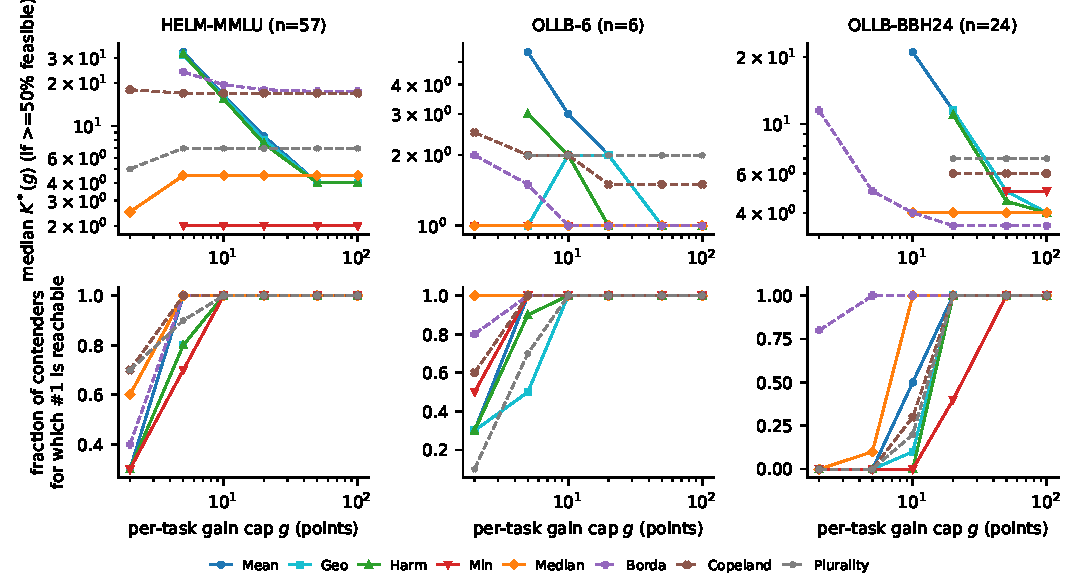
\includegraphics[width=\textwidth]{figs/fig_cap_sweep.pdf}
\caption{Requirement as a function of the per-task cap $g$ for contenders of rank 2--11. Top: median breadth $K^\ast(g)$ (shown when at least half of the contenders can win). Bottom: share of contenders for which first place is reachable.}\label{fig:cap}
\end{figure}

\begin{figure}[h]
\centering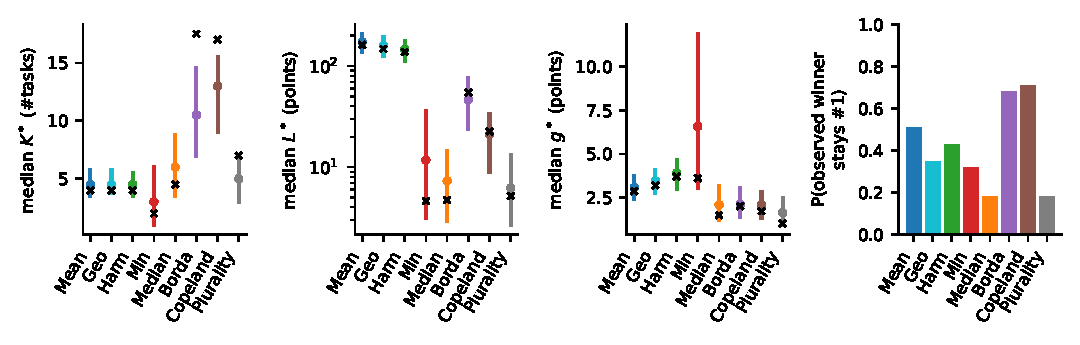
\includegraphics[width=0.45\textwidth]{figs/fig_noise.pdf}\hfill
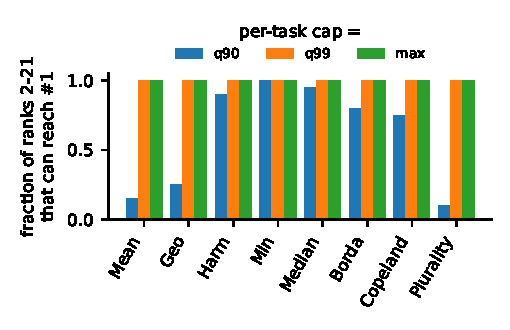
\includegraphics[width=0.45\textwidth]{figs/fig_calibrated.pdf}
\caption{Left: score-noise bootstrap on HELM (bars: 95\% interval over draws; dots: median; crosses: observed). Right: share of OLLB-6 ranks 2--21 that can reach first place under calibrated caps (primary pair set).}\label{fig:noisecal}
\end{figure}

\section{Reproducibility}\label{app:repro}
The repository README lists the environment (Python 3.11, NumPy 2.4.6, SciPy 1.17.1, pandas 3.0.6, matplotlib 3.11.2, pyarrow 26.0.1), data URLs and SHA-256 checksums (\texttt{data/MANIFEST.json}), seeds, commands, approximate run times, and the script that produces each table and figure. All numbers in the paper are produced by the scripts in \texttt{code/}; no value was typed by hand. Total compute was about 20 CPU-hours on a shared 40-core CPU machine (an upper estimate; larger than the 4 CPU-hour planning estimate because the Monte-Carlo studies use 40--100 repetitions of every board and rule), with no GPU. \textbf{Licences and LLM use.} HELM's code is Apache-2.0; we found no licence statement for its score data, nor for the Open LLM Leaderboard \texttt{results} dataset; the \texttt{contents} card has no licence field but a per-model hub-licence column. We redistribute no raw data: scripts download from the public sources and verify checksums. The study design, code and text were produced by an autonomous LLM-based research agent working unattended, which is a non-standard element of the research process, not of the evaluated methods. We searched the web only for the template, the data, and to verify that cited references exist, and did not look for or read any page outside the permitted starter list. Failed or abandoned runs: the first download of the OLLB \texttt{results} files was rate-limited (HTTP 429) and was repeated with back-off; the first version of the median solver (breakpoint search without exact assignment of the breadth) failed our brute-force test and was replaced before any result was produced; no experiment reported here was dropped.

\newpage
\section*{NeurIPS Paper Checklist}




\begin{enumerate}

\item {\bf Claims}
    \item[] Question: Do the main claims made in the abstract and introduction accurately reflect the paper's contributions and scope?
    \item[] Answer: \answerYes{}
    \item[] Justification: The abstract and introduction state the claims (rule-dependent minimum investment, three cost measures, no uniformly hardest rule) and the assumptions; each claim is supported by a numbered result in Sec.~\ref{sec:results} and the limits are stated in Sec.~6.
    \item[] Guidelines:
    \begin{itemize}
        \item The answer \answerNA{} means that the abstract and introduction do not include the claims made in the paper.
        \item The abstract and/or introduction should clearly state the claims made, including the contributions made in the paper and important assumptions and limitations. A \answerNo{} or \answerNA{} answer to this question will not be perceived well by the reviewers. 
        \item The claims made should match theoretical and experimental results, and reflect how much the results can be expected to generalize to other settings. 
        \item It is fine to include aspirational goals as motivation as long as it is clear that these goals are not attained by the paper. 
    \end{itemize}

\item {\bf Limitations}
    \item[] Question: Does the paper discuss the limitations of the work performed by the authors?
    \item[] Answer: \answerYes{}
    \item[] Justification: Sec.~6 (Discussion and limitations) lists nine limitations, including static rivals, no spillover, noise-free scores, three boards, the exploratory design and the top-100 pool for ordinal rules.
    \item[] Guidelines:
    \begin{itemize}
        \item The answer \answerNA{} means that the paper has no limitation while the answer \answerNo{} means that the paper has limitations, but those are not discussed in the paper. 
        \item The authors are encouraged to create a separate ``Limitations'' section in their paper.
        \item The paper should point out any strong assumptions and how robust the results are to violations of these assumptions (e.g., independence assumptions, noiseless settings, model well-specification, asymptotic approximations only holding locally). The authors should reflect on how these assumptions might be violated in practice and what the implications would be.
        \item The authors should reflect on the scope of the claims made, e.g., if the approach was only tested on a few datasets or with a few runs. In general, empirical results often depend on implicit assumptions, which should be articulated.
        \item The authors should reflect on the factors that influence the performance of the approach. For example, a facial recognition algorithm may perform poorly when image resolution is low or images are taken in low lighting. Or a speech-to-text system might not be used reliably to provide closed captions for online lectures because it fails to handle technical jargon.
        \item The authors should discuss the computational efficiency of the proposed algorithms and how they scale with dataset size.
        \item If applicable, the authors should discuss possible limitations of their approach to address problems of privacy and fairness.
        \item While the authors might fear that complete honesty about limitations might be used by reviewers as grounds for rejection, a worse outcome might be that reviewers discover limitations that aren't acknowledged in the paper. The authors should use their best judgment and recognize that individual actions in favor of transparency play an important role in developing norms that preserve the integrity of the community. Reviewers will be specifically instructed to not penalize honesty concerning limitations.
    \end{itemize}

\item {\bf Theory assumptions and proofs}
    \item[] Question: For each theoretical result, does the paper provide the full set of assumptions and a complete (and correct) proof?
    \item[] Answer: \answerYes{}
    \item[] Justification: Propositions 1--4 state their assumptions; complete proofs are in App.~\ref{app:proofs}. The ordinal MILP encoding is argued in App.~\ref{app:proofs} and checked against brute force.
    \item[] Guidelines:
    \begin{itemize}
        \item The answer \answerNA{} means that the paper does not include theoretical results. 
        \item All the theorems, formulas, and proofs in the paper should be numbered and cross-referenced.
        \item All assumptions should be clearly stated or referenced in the statement of any theorems.
        \item The proofs can either appear in the main paper or the supplemental material, but if they appear in the supplemental material, the authors are encouraged to provide a short proof sketch to provide intuition. 
        \item Inversely, any informal proof provided in the core of the paper should be complemented by formal proofs provided in appendix or supplemental material.
        \item Theorems and Lemmas that the proof relies upon should be properly referenced. 
    \end{itemize}

    \item {\bf Experimental result reproducibility}
    \item[] Question: Does the paper fully disclose all the information needed to reproduce the main experimental results of the paper to the extent that it affects the main claims and/or conclusions of the paper (regardless of whether the code and data are provided or not)?
    \item[] Answer: \answerYes{}
    \item[] Justification: Sec.~\ref{sec:setup}, Sec.~\ref{sec:framework} and App.~\ref{app:repro} give data versions, targets, caps, margins, solver settings and statistics; the README lists commands and seeds.
    \item[] Guidelines:
    \begin{itemize}
        \item The answer \answerNA{} means that the paper does not include experiments.
        \item If the paper includes experiments, a \answerNo{} answer to this question will not be perceived well by the reviewers: Making the paper reproducible is important, regardless of whether the code and data are provided or not.
        \item If the contribution is a dataset and\slash or model, the authors should describe the steps taken to make their results reproducible or verifiable. 
        \item Depending on the contribution, reproducibility can be accomplished in various ways. For example, if the contribution is a novel architecture, describing the architecture fully might suffice, or if the contribution is a specific model and empirical evaluation, it may be necessary to either make it possible for others to replicate the model with the same dataset, or provide access to the model. In general. releasing code and data is often one good way to accomplish this, but reproducibility can also be provided via detailed instructions for how to replicate the results, access to a hosted model (e.g., in the case of a large language model), releasing of a model checkpoint, or other means that are appropriate to the research performed.
        \item While NeurIPS does not require releasing code, the conference does require all submissions to provide some reasonable avenue for reproducibility, which may depend on the nature of the contribution. For example
        \begin{enumerate}
            \item If the contribution is primarily a new algorithm, the paper should make it clear how to reproduce that algorithm.
            \item If the contribution is primarily a new model architecture, the paper should describe the architecture clearly and fully.
            \item If the contribution is a new model (e.g., a large language model), then there should either be a way to access this model for reproducing the results or a way to reproduce the model (e.g., with an open-source dataset or instructions for how to construct the dataset).
            \item We recognize that reproducibility may be tricky in some cases, in which case authors are welcome to describe the particular way they provide for reproducibility. In the case of closed-source models, it may be that access to the model is limited in some way (e.g., to registered users), but it should be possible for other researchers to have some path to reproducing or verifying the results.
        \end{enumerate}
    \end{itemize}


\item {\bf Open access to data and code}
    \item[] Question: Does the paper provide open access to the data and code, with sufficient instructions to faithfully reproduce the main experimental results, as described in supplemental material?
    \item[] Answer: \answerYes{}
    \item[] Justification: All code and a README with environment, download scripts, data versions and SHA-256 checksums, seeds, commands, run times and a table-to-script map are provided (anonymised archive); the data are public.
    \item[] Guidelines:
    \begin{itemize}
        \item The answer \answerNA{} means that paper does not include experiments requiring code.
        \item Please see the NeurIPS code and data submission guidelines (\url{https://neurips.cc/public/guides/CodeSubmissionPolicy}) for more details.
        \item While we encourage the release of code and data, we understand that this might not be possible, so \answerNo{} is an acceptable answer. Papers cannot be rejected simply for not including code, unless this is central to the contribution (e.g., for a new open-source benchmark).
        \item The instructions should contain the exact command and environment needed to run to reproduce the results. See the NeurIPS code and data submission guidelines (\url{https://neurips.cc/public/guides/CodeSubmissionPolicy}) for more details.
        \item The authors should provide instructions on data access and preparation, including how to access the raw data, preprocessed data, intermediate data, and generated data, etc.
        \item The authors should provide scripts to reproduce all experimental results for the new proposed method and baselines. If only a subset of experiments are reproducible, they should state which ones are omitted from the script and why.
        \item At submission time, to preserve anonymity, the authors should release anonymized versions (if applicable).
        \item Providing as much information as possible in supplemental material (appended to the paper) is recommended, but including URLs to data and code is permitted.
    \end{itemize}


\item {\bf Experimental setting/details}
    \item[] Question: Does the paper specify all the training and test details (e.g., data splits, hyperparameters, how they were chosen, type of optimizer) necessary to understand the results?
    \item[] Answer: \answerYes{}
    \item[] Justification: No models are trained. Boards, target sets, caps, seeds, bootstrap sizes and solver limits are specified in Sec.~\ref{sec:setup}, the experiment subsections and App.~\ref{app:repro}.
    \item[] Guidelines:
    \begin{itemize}
        \item The answer \answerNA{} means that the paper does not include experiments.
        \item The experimental setting should be presented in the core of the paper to a level of detail that is necessary to appreciate the results and make sense of them.
        \item The full details can be provided either with the code, in appendix, or as supplemental material.
    \end{itemize}

\item {\bf Experiment statistical significance}
    \item[] Question: Does the paper report error bars suitably and correctly defined or other appropriate information about the statistical significance of the experiments?
    \item[] Answer: \answerYes{}
    \item[] Justification: Medians with IQRs over targets, Wilcoxon signed-rank tests with Holm correction, bootstrap intervals over targets, and bootstrap/subsampling/synthetic replicates are reported; what each interval captures is stated. The core computations are deterministic given the board.
    \item[] Guidelines:
    \begin{itemize}
        \item The answer \answerNA{} means that the paper does not include experiments.
        \item The authors should answer \answerYes{} if the results are accompanied by error bars, confidence intervals, or statistical significance tests, at least for the experiments that support the main claims of the paper.
        \item The factors of variability that the error bars are capturing should be clearly stated (for example, train/test split, initialization, random drawing of some parameter, or overall run with given experimental conditions).
        \item The method for calculating the error bars should be explained (closed form formula, call to a library function, bootstrap, etc.)
        \item The assumptions made should be given (e.g., Normally distributed errors).
        \item It should be clear whether the error bar is the standard deviation or the standard error of the mean.
        \item It is OK to report 1-sigma error bars, but one should state it. The authors should preferably report a 2-sigma error bar than state that they have a 96\% CI, if the hypothesis of Normality of errors is not verified.
        \item For asymmetric distributions, the authors should be careful not to show in tables or figures symmetric error bars that would yield results that are out of range (e.g., negative error rates).
        \item If error bars are reported in tables or plots, the authors should explain in the text how they were calculated and reference the corresponding figures or tables in the text.
    \end{itemize}

\item {\bf Experiments compute resources}
    \item[] Question: For each experiment, does the paper provide sufficient information on the computer resources (type of compute workers, memory, time of execution) needed to reproduce the experiments?
    \item[] Answer: \answerYes{}
    \item[] Justification: App.~\ref{app:repro}: CPU only (shared 40-core machine, no GPU), about 20 CPU-hours in total (upper estimate), which exceeded the 4 CPU-hour planning estimate; abandoned or failed runs are listed.
    \item[] Guidelines:
    \begin{itemize}
        \item The answer \answerNA{} means that the paper does not include experiments.
        \item The paper should indicate the type of compute workers CPU or GPU, internal cluster, or cloud provider, including relevant memory and storage.
        \item The paper should provide the amount of compute required for each of the individual experimental runs as well as estimate the total compute. 
        \item The paper should disclose whether the full research project required more compute than the experiments reported in the paper (e.g., preliminary or failed experiments that didn't make it into the paper). 
    \end{itemize}
    
\item {\bf Code of ethics}
    \item[] Question: Does the research conducted in the paper conform, in every respect, with the NeurIPS Code of Ethics \url{https://neurips.cc/public/EthicsGuidelines}?
    \item[] Answer: \answerYes{}
    \item[] Justification: The study uses only public aggregate scores and does not involve human subjects, personal data or model training; we reviewed the Code of Ethics and see no deviation.
    \item[] Guidelines:
    \begin{itemize}
        \item The answer \answerNA{} means that the authors have not reviewed the NeurIPS Code of Ethics.
        \item If the authors answer \answerNo, they should explain the special circumstances that require a deviation from the Code of Ethics.
        \item The authors should make sure to preserve anonymity (e.g., if there is a special consideration due to laws or regulations in their jurisdiction).
    \end{itemize}


\item {\bf Broader impacts}
    \item[] Question: Does the paper discuss both potential positive societal impacts and negative societal impacts of the work performed?
    \item[] Answer: \answerYes{}
    \item[] Justification: Broader impact paragraph in Sec.~6: the analysis could inform benchmark design (positive) and could in principle guide gaming (negative); the case study is descriptive and makes no claim about specific developers.
    \item[] Guidelines:
    \begin{itemize}
        \item The answer \answerNA{} means that there is no societal impact of the work performed.
        \item If the authors answer \answerNA{} or \answerNo, they should explain why their work has no societal impact or why the paper does not address societal impact.
        \item Examples of negative societal impacts include potential malicious or unintended uses (e.g., disinformation, generating fake profiles, surveillance), fairness considerations (e.g., deployment of technologies that could make decisions that unfairly impact specific groups), privacy considerations, and security considerations.
        \item The conference expects that many papers will be foundational research and not tied to particular applications, let alone deployments. However, if there is a direct path to any negative applications, the authors should point it out. For example, it is legitimate to point out that an improvement in the quality of generative models could be used to generate Deepfakes for disinformation. On the other hand, it is not needed to point out that a generic algorithm for optimizing neural networks could enable people to train models that generate Deepfakes faster.
        \item The authors should consider possible harms that could arise when the technology is being used as intended and functioning correctly, harms that could arise when the technology is being used as intended but gives incorrect results, and harms following from (intentional or unintentional) misuse of the technology.
        \item If there are negative societal impacts, the authors could also discuss possible mitigation strategies (e.g., gated release of models, providing defenses in addition to attacks, mechanisms for monitoring misuse, mechanisms to monitor how a system learns from feedback over time, improving the efficiency and accessibility of ML).
    \end{itemize}
    
\item {\bf Safeguards}
    \item[] Question: Does the paper describe safeguards that have been put in place for responsible release of data or models that have a high risk for misuse (e.g., pre-trained language models, image generators, or scraped datasets)?
    \item[] Answer: \answerYes{}
    \item[] Justification: No models or scraped datasets with misuse risk are released.
    \item[] Guidelines:
    \begin{itemize}
        \item The answer \answerNA{} means that the paper poses no such risks.
        \item Released models that have a high risk for misuse or dual-use should be released with necessary safeguards to allow for controlled use of the model, for example by requiring that users adhere to usage guidelines or restrictions to access the model or implementing safety filters. 
        \item Datasets that have been scraped from the Internet could pose safety risks. The authors should describe how they avoided releasing unsafe images.
        \item We recognize that providing effective safeguards is challenging, and many papers do not require this, but we encourage authors to take this into account and make a best faith effort.
    \end{itemize}

\item {\bf Licenses for existing assets}
    \item[] Question: Are the creators or original owners of assets (e.g., code, data, models), used in the paper, properly credited and are the license and terms of use explicitly mentioned and properly respected?
    \item[] Answer: \answerYes{}
    \item[] Justification: Assets are cited with versions and URLs (HELM v1.13.0, code Apache-2.0; Open LLM Leaderboard snapshots by commit). Licences for the score data are not declared; this is stated in App.~\ref{app:repro} and only aggregate scores are used.
    \item[] Guidelines:
    \begin{itemize}
        \item The answer \answerNA{} means that the paper does not use existing assets.
        \item The authors should cite the original paper that produced the code package or dataset.
        \item The authors should state which version of the asset is used and, if possible, include a URL.
        \item The name of the license (e.g., CC-BY 4.0) should be included for each asset.
        \item For scraped data from a particular source (e.g., website), the copyright and terms of service of that source should be provided.
        \item If assets are released, the license, copyright information, and terms of use in the package should be provided. For popular datasets, \url{paperswithcode.com/datasets} has curated licenses for some datasets. Their licensing guide can help determine the license of a dataset.
        \item For existing datasets that are re-packaged, both the original license and the license of the derived asset (if it has changed) should be provided.
        \item If this information is not available online, the authors are encouraged to reach out to the asset's creators.
    \end{itemize}

\item {\bf New assets}
    \item[] Question: Are new assets introduced in the paper well documented and is the documentation provided alongside the assets?
    \item[] Answer: \answerYes{}
    \item[] Justification: The released code is documented in the README (what each script does, inputs, outputs, run times). No new dataset is released apart from small derived result tables.
    \item[] Guidelines:
    \begin{itemize}
        \item The answer \answerNA{} means that the paper does not release new assets.
        \item Researchers should communicate the details of the dataset\slash code\slash model as part of their submissions via structured templates. This includes details about training, license, limitations, etc. 
        \item The paper should discuss whether and how consent was obtained from people whose asset is used.
        \item At submission time, remember to anonymize your assets (if applicable). You can either create an anonymized URL or include an anonymized zip file.
    \end{itemize}

\item {\bf Crowdsourcing and research with human subjects}
    \item[] Question: For crowdsourcing experiments and research with human subjects, does the paper include the full text of instructions given to participants and screenshots, if applicable, as well as details about compensation (if any)? 
    \item[] Answer: \answerYes{}
    \item[] Justification: No crowdsourcing or human subjects.
    \item[] Guidelines:
    \begin{itemize}
        \item The answer \answerNA{} means that the paper does not involve crowdsourcing nor research with human subjects.
        \item Including this information in the supplemental material is fine, but if the main contribution of the paper involves human subjects, then as much detail as possible should be included in the main paper. 
        \item According to the NeurIPS Code of Ethics, workers involved in data collection, curation, or other labor should be paid at least the minimum wage in the country of the data collector. 
    \end{itemize}

\item {\bf Institutional review board (IRB) approvals or equivalent for research with human subjects}
    \item[] Question: Does the paper describe potential risks incurred by study participants, whether such risks were disclosed to the subjects, and whether Institutional Review Board (IRB) approvals (or an equivalent approval/review based on the requirements of your country or institution) were obtained?
    \item[] Answer: \answerYes{}
    \item[] Justification: No human subjects.
    \item[] Guidelines:
    \begin{itemize}
        \item The answer \answerNA{} means that the paper does not involve crowdsourcing nor research with human subjects.
        \item Depending on the country in which research is conducted, IRB approval (or equivalent) may be required for any human subjects research. If you obtained IRB approval, you should clearly state this in the paper. 
        \item We recognize that the procedures for this may vary significantly between institutions and locations, and we expect authors to adhere to the NeurIPS Code of Ethics and the guidelines for their institution. 
        \item For initial submissions, do not include any information that would break anonymity (if applicable), such as the institution conducting the review.
    \end{itemize}

\item {\bf Declaration of LLM usage}
    \item[] Question: Does the paper describe the usage of LLMs if it is an important, original, or non-standard component of the core methods in this research? Note that if the LLM is used only for writing, editing, or formatting purposes and does \emph{not} impact the core methodology, scientific rigor, or originality of the research, declaration is not required.
    %this research? 
    \item[] Answer: \answerYes{}
    \item[] Justification: The research (study design, code and drafting) was carried out by an autonomous LLM-based research agent; this is declared in App.~\ref{app:repro}. LLMs are not a component of the evaluated methods.
    \item[] Guidelines:
    \begin{itemize}
        \item The answer \answerNA{} means that the core method development in this research does not involve LLMs as any important, original, or non-standard components.
        \item Please refer to our LLM policy in the NeurIPS handbook for what should or should not be described.
    \end{itemize}

\end{enumerate}
\end{document}
